include(`macros.m4')

\pagebreak
\pdfbookmark[0]{access rights, peripheral devices, file system}{user access}

\begin{slide}
\sltitle{Contents}
\slidecontents{3}
\end{slide}

\begin{slide}
\sltitle{Users and groups}
\begin{center}
\framebox{\texttt{beran:x:1205:106:Martin Beran:/home/beran:/bin/bash}}
\end{center}
\vspace{2ex}

\emsl{The fields, in order from left to right:} user name, 
hashed password (today in \texttt{/etc/shadow} or elsewhere), user ID (aka UID);
primary group ID (aka GID), full name, home directory, login shell

Note that a superuser (root) has always UID 0.

\vspace{2ex}
\begin{center}
\framebox{\texttt{sisal:*:106:forst,beran}}
\end{center}
\vspace{2ex}

\emsl{The fields, in order from left to right:} group name, group password (not
used today), group ID (GID), list of group members
\end{slide}

\begin{itemize}
\item User information in files \texttt{/etc/passwd} and \texttt{/etc/group} are
processed by various system programs, like \texttt{login} or \texttt{su}.
The kernel knows nothing about these files as it only uses numeric
representation of users and groups.
\item Passwords are long gone from \texttt{/etc/passwd}, they are stored some
place else, for example in \texttt{/etc/shadow}, which is not readable to an
unprivileged user.  The passwords are also salted and then hashed. On BSD based
systems, e.g. FreeBSD or macOS, instead of \texttt{/etc/shadow},
\texttt{/etc/master.passwd} database is used.
\item If \texttt{/etc/shadow} does exist, it is structured in a similar way as
\texttt{/etc/passwd}.
\item There are also protocols used for authentication that do not use
\texttt{/etc/passwd} at all, for example NIS (Network Information Service) or
LDAP (Lightweight Directory Access Protocol).
\item The user group in \texttt{/etc/passwd} is called \emph{primary} for the
user.  Such a group is used when files are created.  Other groups a user belongs
to, those in the user's entry in \texttt{/etc/group}, are called
\emph{supplementary} and provide additional group privileges to access files.
\end{itemize}

%%%%%

\pdfbookmark[1]{file access rights}{fsaccessrights}

\begin{slide}
\sltitle{Access rights}
\begin{center}
\begin{picture}(0,0)%
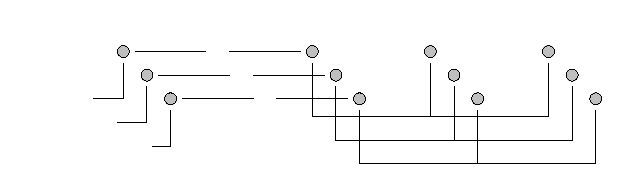
\includegraphics{img/tex/access_rights}%
\end{picture}%
\setlength{\unitlength}{4144sp}%
%
\begingroup\makeatletter\ifx\SetFigFont\undefined%
\gdef\SetFigFont#1#2#3#4#5{%
  \reset@font\fontsize{#1}{#2pt}%
  \fontfamily{#3}\fontseries{#4}\fontshape{#5}%
  \selectfont}%
\fi\endgroup%
\begin{picture}(4463,1155)(226,-466)
\put(4096,569){\makebox(0,0)[lb]{\smash{\SetFigFont{10}{12.0}{\sfdefault}{\mddefault}{\updefault}{\color[rgb]{0,0,0}$\stackrel{\mbox{others (o)}}{\overbrace{\hphantom{\hspace{1cm}}}}$}%
}}}
\put(3196,569){\makebox(0,0)[lb]{\smash{\SetFigFont{10}{12.0}{\sfdefault}{\mddefault}{\updefault}{\color[rgb]{0,0,0}$\stackrel{\mbox{group (g)}}{\overbrace{\hphantom{\hspace{1cm}}}}$}%
}}}
\put(2296,569){\makebox(0,0)[lb]{\smash{\SetFigFont{10}{12.0}{\sfdefault}{\mddefault}{\updefault}{\color[rgb]{0,0,0}$\stackrel{\mbox{owner (u)}}{\overbrace{\hphantom{\hspace{1cm}}}}$}%
}}}
\put(1711,389){\makebox(0,0)[lb]{\smash{\SetFigFont{10}{12.0}{\sfdefault}{\mddefault}{\updefault}{\color[rgb]{0,0,0}4}%
}}}
\put(1891,209){\makebox(0,0)[lb]{\smash{\SetFigFont{10}{12.0}{\sfdefault}{\mddefault}{\updefault}{\color[rgb]{0,0,0}2}%
}}}
\put(2071, 29){\makebox(0,0)[lb]{\smash{\SetFigFont{10}{12.0}{\sfdefault}{\mddefault}{\updefault}{\color[rgb]{0,0,0}1}%
}}}
\put(541, 29){\makebox(0,0)[lb]{\smash{\SetFigFont{10}{12.0}{\sfdefault}{\mddefault}{\updefault}{\color[rgb]{0,0,0}SUID}%
}}}
\put(721,-151){\makebox(0,0)[lb]{\smash{\SetFigFont{10}{12.0}{\sfdefault}{\mddefault}{\updefault}{\color[rgb]{0,0,0}SGID}%
}}}
\put(901,-331){\makebox(0,0)[lb]{\smash{\SetFigFont{10}{12.0}{\sfdefault}{\mddefault}{\updefault}{\color[rgb]{0,0,0}sticky}%
}}}
\put(226,389){\makebox(0,0)[lb]{\smash{\SetFigFont{10}{12.0}{\sfdefault}{\mddefault}{\updefault}{\color[rgb]{0,0,0}highest bit}%
}}}
\put(2341,-106){\makebox(0,0)[lb]{\smash{\SetFigFont{10}{12.0}{\sfdefault}{\mddefault}{\updefault}{\color[rgb]{0,0,0}r}%
}}}
\put(2521,-286){\makebox(0,0)[lb]{\smash{\SetFigFont{10}{12.0}{\sfdefault}{\mddefault}{\updefault}{\color[rgb]{0,0,0}w}%
}}}
\put(2701,-466){\makebox(0,0)[lb]{\smash{\SetFigFont{10}{12.0}{\sfdefault}{\mddefault}{\updefault}{\color[rgb]{0,0,0}x}%
}}}
\end{picture}

\end{center}
\begin{itemize}
\item \emsl{SGID} on a file without the executable bit for its group means
\emsl{mandatory locking} in systems based on System~V
\item \emsl{sticky bit} for directories: remove and renamed allowed for file
owners only.
\item \emsl{SGID} for directory: new files will have the same group as the
directory (on System~V based systems; it works in a different way on BSD
systems, see below)
\end{itemize}
\end{slide}

\begin{itemize}
\item The sticky bit for directories means that when the directory is writable
for a given user (possibly because all users can write), the user can create any
file that does not exist in that directory yet.  However, if the file exists but
is not owned by the user, he/she can not remove nor rename it even if
he/she can write the directory.  The sticky bit is denoted by ``t'' and is
typically used for temporary directories:

\begin{verbatim}
$ ls -ld /tmp
drwxrwxrwt 9 root root 356352 Jan 27 22:37 /tmp/
\end{verbatim}

\item The SGID bit for directories on BSD based systems means that files and
directories created in this directory will have the same owner as the directory
itself.  The filesystem must be mounted with an \texttt{suiddir} flag and
the kernel may need an additional non-default option \texttt{SUIDDIR}.  It also
does not work for the root user.  This functionality is there to support Samba.
\item Originally, the sticky bit had a meaning for regular files as well but
that is not used anymore.
\item Some filesystems (XFS, AFS, UFS2, ZFS, and others) also support
\emph{access control lists} (ACLs) that allow for finer access right management.
\end{itemize}
%%%%%

ifdef([[[NOSPELLCHECK]]], [[[
\pdfbookmark[1]{getpwnam, getpwuid, getpwent}{getpw}
]]])

\label{GETPW_FUNC}
\begin{slide}
\sltitle{Obtain user/group information}
\begin{itemize}
ifdef([[[NOSPELLCHECK]]], [[[
\item \texttt{struct passwd *\funnm{getpwnam}(const char *name)}
]]])
return structure describing user found in password database or NULL.

ifdef([[[NOSPELLCHECK]]], [[[
\item \texttt{struct passwd *\funnm{getpwuid}(uid\_t uid)}
]]])
ditto; perform search according to UID.
ifdef([[[NOSPELLCHECK]]], [[[
\item \texttt{void \funnm{setpwent}(void)}
\item \texttt{void \funnm{endpwent}(void)}
\item \texttt{struct passwd *\funnm{getpwent}(void)}
]]])
these functions traverse password database. \funnm{setpwent} rewinds to the
beginning of the password database, \funnm{getpwent} gets the current entry,
\funnm{endpwent} closes the password database and free allocated resources.
\end{itemize}
\end{slide}

\begin{itemize}
\item These functions work independently on what database was used to get the
user information, see page \pageref{name_service_switch} for more information on
naming databases.
\item All these functions are part of POSIX 1003.1-2008.
\item \funnm{setpwent}() must be call before the first call to
\funnm{getpwent}().
\item There are also functions \funnm{getgrnam}() and \funnm{getgrent}() which
can be used to get group information.
\item To search and list naming databases, you can use the program \texttt{getent}.
For example:

\begin{verbatim}
$ getent passwd root
root:x:0:0:Super-User:/root:/sbin/sh
$ getent group root
root::0:
\end{verbatim}
\end{itemize}

%%%%%

\pdfbookmark[1]{name service switch}{NSS}

\begin{slide}
\sltitle{Name service switch}
\begin{itemize}
\item today's systems are not confined to only using
\texttt{/etc/passwd} and \texttt{/etc/groups}
\item such systems have \emph{databases} (\texttt{passwd, groups, protocols},
\dots)
\item database data come from \emph{sources} (files, DNS, NIS, LDAP, \dots)
\item file \texttt{nsswitch.conf} defines what databases use what sources
\item library functions must support this, obviously
\item it is possible to combine some sources, e.g. users may be first be searched
in \texttt{/etc/passwd}, then in LDAP
\item came first with Solaris, other systems borrowed the idea
\end{itemize}
\end{slide}

\label{name_service_switch}

\begin{itemize}
\item Systems using the name service switch typically use the
\texttt{nsswitch.conf(4)} file to store information about what databases
are supported, including the API.  For example, with the \texttt{passwd}
database, standard calls like \texttt{getpwnam(3)} and \texttt{getpwent(3)} use
it.  In general, it is not needed to process such databases manually, as there is
always an API to use for that.
\item Example of an existing \texttt{nsswitch.conf} on Solaris:

\begin{verbatim}
passwd:     files ldap
group:      files ldap

# You must also set up the /etc/resolv.conf file for DNS name
# server lookup.  See resolv.conf(4).
hosts:      files dns

# Note that IPv4 addresses are searched for in all of the
# ipnodes databases before searching the hosts databases.
ipnodes:   files dns

networks:   files
protocols:  files
rpc:        files
ethers:     files
\end{verbatim}
\end{itemize}

%%%%%

\pdfbookmark[1]{Access rights evaluation algorithm}{accessrights}

\begin{slide}
\sltitle{Access rights testing}
\setlength{\baselineskip}{0.9\baselineskip}
\begin{itemize}
\item a user is identified with a \emsl{UID} number and numbers for groups he
belongs to (\emsl{primary GID}, \emsl{supplementary GIDs})
\item this identification is inherited by each process
\item file $F$ has owner ($UID_F$) and group owner ($GID_F$). 
\item the algorithm for evaluation of access rights for process:
ifdef([[[NOSPELLCHECK]]], [[[$P(UID_P,GID_P,SUPG)$]]]) and file
ifdef([[[NOSPELLCHECK]]], [[[$F(UID_F,GID_F)$]]]):
\begin{tabular}{ll}
If & then ifdef([[[NOSPELLCHECK]]], [[[$P$rocess]]]) has w.r.t.
ifdef([[[NOSPELLCHECK]]], [[[$F$ile]]]) \\ 
\hline
\texttt{if($UID_P$ == 0)} & \dots{} all rights \\
\texttt{else if($UID_P$ == $UID_F$)} & \dots{} owner rights \\
\texttt{else if($GID_P$ == $GID_F$ ||} &\\
\texttt{~~~~~~~~$GID_F \in SUPG$)} & \dots{} group rights \\
\texttt{else} & \dots{} rights of others
\end{tabular}
\end{itemize}
\end{slide}

\begin{itemize}
\item The processes of the \texttt{root} user can change its user and group
identity. This is used e.g. by the \texttt{login} process, which runs as
\texttt{root} and after performing an authentication check successfully, runs
a shell process with the identity of the given user (using the \texttt{setuid} syscall
-- see upcoming slides).
\item The implication of the algorithm is that for the \texttt{root} user, the
access rights are not relevant (it has always unlimited access -- at least in
classic UNIX without fine grained privileges). If the user is equal, the
group/other rights are not used even though they permit more than what user
rights do. Similarly the others rights are not used if the group is equal.
\emsl{Therefore if a file owned by a user has the rights set to
\texttt{---rwxrwx}, the user cannot read/write/execute it until he/she changes
the rights.}
\item More and more systems diverge from the classic model where many processes
were running under a user with UID 0. A security vulnerability in such an
application meant total control of the system. To thwart this, these systems
employ models like \emph{least privilege} in Solaris or \emph{privilege
separation} and \emph{pledge} in OpenBSD.
\item \label{FILEDELETE} In order to delete a file, the user has to have write
permission for the \emsl{directory} containing the file, because that is actually
the ``file'' being changed. \emsl{The rights of the file to be deleted are
not relevant}; the shell might give you a warning that you are about to delete a
file for which you do not have the right to write, however that is just a
warning, the operation will proceed.  It is quite logical -- if you set a file
as read-only the shell will deduce that you probably do not want to delete such
a file.  See the example below.  \emsl{Unix systems do not have delete-like
operation for a file}, the file is deleted automatically once it is no longer
referenced from a directory structure and the file is not presently open by any
process.

\begin{verbatim}
$ whoami
janp
$ ls -ld janp-dir
drwx------   2 janp  staff  512 Mar 23 12:12 janp-dir/
$ ls -l janp-dir
total 0
-rw-r--r--   1 root  root     0 Mar 23 12:11 root_wuz_here.txt
$ rm janp-dir/root_wuz_here.txt 
rm: janp-dir/root_wuz_here.txt: override protection 644 (yes/no)? yes
$ ls janp-dir/root_wuz_here.txt 
janp-dir/root_wuz_here.txt: No such file or directory
\end{verbatim}

\item However if \texttt{root} creates its own sub-directory in the
\texttt{janp-dir} directory and then creates a new file in there, the
\texttt{janp} user can no longer delete the \texttt{janp-dir} directory and its
contents because:
\begin{itemize}
\item no directory can be deleted if non-empty, and
\item the given file created by \texttt{root} cannot be deleted because
\texttt{janp} is not an owner of the sub-directory containing the file
\end{itemize}
\item If the read bit is removed from a directory rights, it is not possible to
read its contents, therefore you cannot list files contained therein. However if you
know the name of the file in the directory and the execute bit is set, you can
read the file:
\begin{verbatim}
$ mkdir foo
$ ls -ald foo
drwxr-xr-x  2 vladimirkotal  staff  68 Nov  5 14:37 foo
$ touch foo/bar
$ file foo/bar
foo/bar: empty
$ ls foo
bar
$ chmod u-r foo
$ ls foo
ls: foo: Permission denied
$ file foo/bar
foo/bar: empty
\end{verbatim}
\item There is a situation where even the execute bit for a directory is not
sufficient.  That is used for temporary directories where anyone can write to.
However, it is not desirable to permit users to delete each others files.
To achieve that there is the \emph{sticky bit} (01000).  There might be a
\texttt{sticky} man page, where the sticky bit function is described.
It is visible as \texttt{\emsl{t}} in the \texttt{ls} output:

\begin{verbatim}
$ ls -ld /tmp
drwxrwxrwt   7 root     root         515 Mar 23 12:22 /tmp
\end{verbatim}
\end{itemize}

%%%%%

ifdef([[[NOSPELLCHECK]]], [[[
\pdfbookmark[1]{ruid, euid, suid}{resugid}
]]])

\begin{slide}
\sltitle{Real and effective UID/GID}
\begin{itemize}
\item for each process the following IDs are distinguished:
    \begin{itemize}
    \item \emsl{real UID} (RUID) -- real owner of the process
    \item \emsl{effective UID} (EUID) -- user, whose rights are used by the
process
    \item \emsl{saved UID} -- original effective UID
    \end{itemize}
\item similarly each process has the real, effective and saved GID.
\item usually \texttt{RUID==EUID \&\& RGID==EGID}.
\item \emsl{right vesting} \dots{} execution of a program with
the SUID (\emsl{set user ID}) bit set changes the EUID and the saved UID of the process
to the UID of the program owner, the RUID stays the same.
\item similarly the SGID bit changes the EGID of the process. 
\end{itemize}
\end{slide}

\label{ROOT_SETUID}

\begin{itemize}
\item \emsl{access rights checking always consults the EUID, EGID, and
supplementary GIDs}
\item \label{SUID_BIT} The SUID and SGID bits are used for programs that need
bigger privileges than the user who executes them. One example is the
\texttt{passwd} program that needs to update files \texttt{/etc/passwd} and
\texttt{/etc/shadow}, where the ordinary user cannot modify the first and
cannot write into the the second. Another example is the \texttt{su} program,
which has to have the right to arbitrarily change user and group identity,
which is a privilege of programs running with UID~0.
\item Programs using the SUID and SGID bits should be carefully programmed
to allow only the operations for which they were designed and prevent misuse
of their privileges for non-authorized actions (root shell execution).
Such programs used to be one of the most frequent causes of security problems
in Unix systems.
\item The basic rule for writing SUID/SGID programs is: \emsl{do not write
them} if it is not absolutely necessary.  It is not easy to produce a correct
(i.e. secure) SUID/SGID program, especially of higher complexity.
\item \emsl{These are the rules for ID change:}
\begin{itemize}
\item an ordinary user cannot change its RUID or saved UID (the \texttt{exec} is
an exception to that, see page \pageref{EXEC})
\item the process can always change its EUID to that of the RUID or saved UID.
This guarantees that in a SUID program, it is possible to arbitrarily change the EUID
between the one that enabled the process to gain ownership rights and the
UID of the real user that executed the process originally.
\item \emsl{root can do everything}, and when it changes the RUID, it will also
change saved the UID -- it does not make sense to change just one of them when
either can be used to set the EUID.
\end{itemize}
\end{itemize}

%%%%%
 
ifdef([[[NOSPELLCHECK]]], [[[
\pdfbookmark[1]{getuid, getgid, geteuid, getegid, getgroups}{getuid}
]]])

\begin{slide}
\sltitle{Process owner identification}
\begin{itemize}
ifdef([[[NOSPELLCHECK]]], [[[
\item \texttt{uid\_t \funnm{getuid}(void)}
]]])
returns the real user ID of the calling process.
ifdef([[[NOSPELLCHECK]]], [[[
\item \texttt{uid\_t \funnm{geteuid}(void)}
]]])
returns the effective user ID of the calling process.
ifdef([[[NOSPELLCHECK]]], [[[
\item \texttt{gid\_t \funnm{getgid}(void)}
]]])
returns the real group ID of the calling process.
ifdef([[[NOSPELLCHECK]]], [[[
\item \texttt{gid\_t \funnm{getegid}(void)}
]]])
returns the effective group ID of the calling process.
ifdef([[[NOSPELLCHECK]]], [[[
\item \texttt{int \funnm{getgroups}(int \emph{gidsz}, gid\_t \emph{glist}[])}
]]])
-- \texttt{glist} returns at most \texttt{gidsz} supplementary group
IDs of the calling process and returns number of all GIDs of the process.
\end{itemize}
\end{slide}

\begin{itemize}
\item The \texttt{getuid} returns real the UID, there is nothing like
\texttt{getruid}.
\item \texttt{getgroups}: when \texttt{gidsz~==~0}, it returns the number of
groups. When \texttt{0 < gidsz < \#groups}, it returns \texttt{-1}.
\item In Unix, there are many data types such as \verb#uid_t#, \verb#gid_t#,
\verb#size_t#, \verb#pid_t#, etc.  In general, these are integer types and you
can often find them in the
ifdef([[[NOSPELLCHECK]]], [[[\texttt{/usr/inc{}lude/sys/types.h}]]]) header
file.
\item Solaris has the \texttt{pcred} command that provides process
identification information in a simple form:

\begin{verbatim}
$ pcred 5464
5464:   e/r/suid=1993  e/r/sgid=110
        groups: 33541 41331 110
\end{verbatim}
\end{itemize}

%%%%%

ifdef([[[NOSPELLCHECK]]], [[[
\pdfbookmark[1]{setuid, setgid, setgroups}{ownerchange}
]]])

\begin{slide}
\sltitle{Process owner change}
\begin{itemize}
ifdef([[[NOSPELLCHECK]]], [[[
\item \texttt{int \funnm{setuid}(uid\_t \emph{uid});}
]]])
    \begin{itemize}
    \item for a process with EUID~==~0, sets the RUID, EUID and saved-SUID to
    \texttt{uid}
    \item for other processes it sets just the EUID, and \texttt{uid} must be
    either equal to the RUID or saved UID
    \end{itemize}
ifdef([[[NOSPELLCHECK]]], [[[
\item \texttt{int \funnm{setgid}(gid\_t \emph{gid});} \\
]]])
similar to \texttt{setuid}, for group-IDs of the process.
ifdef([[[NOSPELLCHECK]]], [[[
\item \texttt{int \funnm{setgroups}(int \emph{ngroups},
gid\_t *\emph{gidset})} \\
]]])
sets the supplementary group IDs for the calling process. Can only be used
by superuser process.
\end{itemize}
\end{slide}

\begin{itemize}
\item W.r.t. setting the UID for a process with EUID == 0, see also the notes on
page \pageref{ROOT_SETUID}.
\item To recap the above: a process with effective rights of a superuser can
arbitrarily change its identity. The rest can only switch between its real and
effective IDs.
\item The \emph{login} program uses the \texttt{setuid} syscall.
\item If a process with UID~==~0 wants to change its identity, it has to call
\texttt{setgid} first and then \texttt{setgroups}. Only after that can it call
\texttt{setuid}. Any other ordering would mean that the process would lack the
rights to perform the operation in question, e.g. once \texttt{setuid} returns
it would not have the rights to perform \texttt{setgid} and \texttt{setgroups}.
\item \texttt{setgroups} is not part of UNIX~98 or UNIX~03.
\item RUID/EUID are saved in the kernel process structure and also in the so
called \emph{u-area} (see e.g. [Bach]).
\item If a root SUID program calls \texttt{setuid} for a UID other than 0, it
can no longer return the EUID to 0 (this makes sense, imagine a user logging
into the system). For a different behavior, \texttt{seteuid} (that sets just the
EUID) would have to be used.
\item Example: \example{setuid/screate-file.c}
\end{itemize}

\endinput
